\chapter{Resultados dos testes}


\section{Avaliação da Interface}

questionario 1, perfil de cada usuario. Definir como user 1 2 e 3;
resultado etiquetas, pra user 1, 2 e 3.
resultado questionario pra user 1, 2 e 3.

\begin{table}[h!]
  \centering
  \caption{Contabilização das etiquetas para cada usuário. Cada etiqueta é registrada no tempo do vídeo em que ela ocorreu.}
  \label{tabEtiquetas}
  \begin{tabular}{|l|c|c|c|}
  \hline
  {\cellcolor[HTML]{DFDFDF}Etiquetas} & {\cellcolor[HTML]{DFDFDF}Usuário 1} & {\cellcolor[HTML]{DFDFDF}Usuário 2} & {\cellcolor[HTML]{DFDFDF}Usuário 3} \\ \hline
  Desisto. & - & - & - \\ \hline
  Para mim está bom... & - & - & - \\ \hline
  Não, obrigado. & - & - & - \\ \hline
  Vai de outro jeito. & - & - & - \\ \hline
  Cadê? & (01:22), (07:49) & (04:55) & - \\ \hline
  Ué, o que houve? & (09:30) & - & - \\ \hline
  E agora? & - & (02:01) & (01:46) \\ \hline
  Onde estou? & - & - & - \\ \hline
  Epa! & (09:01) & (00:41), (09:30), (10:45) & - \\ \hline
  Assim não dá. & (5:10) & (01:29) & (01:05) \\ \hline
  O que é isto? & (01:26), (03:50) & (02:20), (08:18) & (01:59) \\ \hline
  Socorro! & (01:55), (07:53), (10:15) & (07:55), (10:01) & (06:00), (07:25) \\ \hline
  Por que não funciona? & - & - & (04:20), (07:20) \\ \hline
  \end{tabular}
\end{table}

Usuario 1
\begin{itemize}
\item[01:22] Usuário não encontrou as reações que a enzima catalisada, mas logo percebeu que deveria seguir para uma outra página para obter detalhes sobre a busca;
\item[01:26] Usuário se deparou com um grafo em movimento, com 6 nós e cinco arestas, e não entendeu seu significado, a princípio;
\item[01:55] Usuário precisou interagir com o grafo de maneira forçada, pois o mesmo não parava de se mover;
\item[03:50] Usuário fala "Nossa, isso é muito ruim; Não dá pra saber se o substrato da enzima é verde (Composto) ou o rosa (Reação)";
\item[05:10] Usuário tenta entender a legenda do grafo, mas discorda totalmente do proposto;
\item[07:49] Usuário não encontra informação que buscava, até descobrir que deveria seguir para página de detalhes de busca, novamente;
\item[07:53] Usuário expressa desgosto pelo grafo fechado que aparece ao iniciar a página de detalhes da via metabólica;
\item[09:30] Usuário esqueceu de selecionar \textit{Search} e percebeu que havia selecionado em ver detalhes da busca anterior;
\item[10:15] Usuário logo clica no grafo para ele parar de se mover.
\end{itemize}


Usuario 2
\begin{itemize}
\item[00:41] Usuário percebeu que havia selecionado um botão que não o levava ao seu objetivo;
\item[01:29] Usuário se confunde com função auto-complete do campo de enzimas;
\item[02:01] Usuário demora alguns segundos para perceber que deve seguir para a página de detalhes de busca;
\item[02:20] Usuário demora alguns segundos para entender, a partir da legenda, o significado do grafo que aparece na página de detalhes de busca.
\item[04:55] Usuário não percebe que página retornou sucesso, pois não parece que ela foi atualizada;
\item[07:55] Usuário tenta impedir grafo de se mover para fora de seu campo de visão;
\item[08:18] Usuário tem dificuldade para entender significado biológico das arestas e nós do grafo;
\item[09:30] Usuário esqueceu de selecionar \textit{Search} e percebeu que havia selecionado em ver detalhes da busca anterior;
\item[10:01] Usuário tenta impedir grafo de se mover para fora de seu campo de visão;
\item[10:45] Usuário percebeu que havia errado a tarefa anterior e voltou para refazê-la.
\end{itemize}

Usuario 3
\begin{itemize}
\item[01:05] Usuário se confunde com função auto-complete do campo de enzimas. Ainda percebe que o problema não é o teclado, mas sim a função que aparece sem necessidade e atrapalha a busca;
\item[01:46] Usuário diz "É só essa a informação?", pois não percebeu, a princípio, que para realizar a tarefa deveria seguir para a página de detalhes da busca;
\item[01:59] Usuário não entende grafo que aparece na tela de detalhes e reclama muito por ele não ficar parado;
\item[04:20] Usuário reclama da falta de respostas da interface;
\item[06:00] Usuário acha um absurdo o tamanho do grafo que aparece na tela e pede a lista dos detalhes que ele gostaria de saber sobre a busca;
\item[07:20] Usuário reclama da falta de respostas da interface;
\item[07:25] Usuário acha um absurdo o tamanho do grafo que aparece na tela e pede a lista dos detalhes que ele gostaria de saber sobre a busca.
\end{itemize}









Conclusão:



Aplicação do método da avaliação da comunicabilidade

Pontos fortes: \\

\begin{itemize}
  \item Os botões do menu ao topo do site facilitaram a navegação pelo site;
  \item A função auto-complete dos compostos facilitou muito a busca;
  \item A mensagem de sucesso ou fracasso sempre era reparada.
\end{itemize}

 
Pontos fracos:\\

\begin{itemize}
\item Busca
  \begin{itemize}
  \item[1] O botão de voltar um página, do navegador, não fazia o que o usuário esperava. Ele voltava para a pesquisa anterior ao invés de ir para a página central de buscas;
  \item[2] A função auto-complete das enzimas não foi uma boa decisão de projeto, pois os usuários ficavam confusos com os números que apareciam;
  \item[3] Resultado de busca não estava sendo inicializado toda vez que página é carregada, portanto apresentava um resultado anterior, o que causava confusão;
  \item[4] Botão "View Interative Data", para visualizar a via metabólica, esta sempre ativo. Isso fez com que os usuários não notassem que existe informação extra sobre enzima ou via quando a pesquisa retorna sucesso;
  \item[5] Botões "Search" e "View Interative Data" estavam muito pertos um do outro. Muitos usuários não selecionavam o botão \textit{Search} antes de clicar em "View Interative Data", pois a segunda coluna da página estava mal localizada, para um formulário;
  \item[6] A página de busca central dá mais foco em busca por elementos no organismo, e isso faz com que a seção menor à esquerda passe despercebida.
  \end{itemize}

\item Grafo
  \begin{itemize}
  \item[1] A reação não deveria ser representada por um nó, pois para os biólogos, ela é uma ação, e não um elemento. Assim, faz mais sentido biológico representar COMPOUND-[SUBSTRACT]->ENZIME e ENZIME-[PRODUCTOF]->COMPUND. A aresta "CATALISE" não é necessária. Houve muita confusão, pois pensaram que reação era representada por aresta invés de nó;
  \item[2] Não é necessário apresentar os nós do organismo e sequências que o organismo possui. Ao apresentar a enzima na busca de informações no organismo, já é implícito que aquela enzima é produzida pelo organismo;
  \item[3] Quanto maior o grafo, mais complexo é entendê-los;
  \item[4] Grafos muito grades podem ficar cortados e alguns elementos podem sair do campo de visão do usuário.
  \item[5] É mais desejável um grafo que apareça primeiramente de maneira estática. Um grafo que aparece se movendo levemente é irritante. Caso o usuário queira mover e clicar nos elementos, ele o faz com mais facilidade com um grafo estático;
  \item[6] É mais agradável um grafo que apareça aberto;
  \item[7] As labels poderiam apresentar só as bolinhas e explicação a respeito do que elas representam. A informação sobre as arestas já é informação extra desnecessária;
  \end{itemize}
\end{itemize}


Foi encontrado um \textit{erro} de implementação em um dos testes. Uma das tarefas era encontrar uma via metabólica entre dois compostos no grafo completo do 2Path, porém um dos usuários utilizou a busca por via em um organismo. A busca deveria retornar que não há via, porém ela retornou que existia, e apresentou um grafo disjunto\footnote{Dois grafos que não se conectam.}. Um grafo era do organismo com todas as enzimas que ele produzia e o outro grafo representava a via entre os compostos pesquisados.


Mudanças no projeto de interface após os testes:
\begin{itemize}
\item Busca
  \begin{itemize}
  \item[1] Foi adicionado um botão de voltar nas páginas específicas de busca por enzima e vias metabólicas, assim o usuário pode clicar nele e voltar diretamente para a página de buscas gerais;
  \item[2] A função \textit{auto-complete} do campo de busca por enzima foi removido;
  \item[3] As mensagens de sucesso e erro são apresentadas no canto superior direito da tela e são atualizadas sempre que uma nova busca é feita. Ela aparece por 5 segundos e depois desaparece.
  \item[4, 5] O grafo que apresenta os detalhes sobre a enzima ou via metabólica buscada aparece na mesma página que o formulário de pesquisa. Se a busca retorna verdadeira, o grafo aparece, se retorna falsa, não aparece. Assim, o usuário não precisa seguir mais um passo na interface para visualizar os dados biológicos que procura;
  \item[6] As colunar de busca no banco completo e no organismo foram configuradas no mesmo tamanho e ícones que simbolizam elementos públicos e privados foram posicionados ao lado dos títulos de cada busca.
  \end{itemize}
  
\item Grafo
  \begin{itemize} 
  \item[1] NÃO DÁ: Uma enzima pode catalisar mais de uma reação. Assim, não teria como representar o nó da enzima recebendo todos os possíveis substratos e produzindo todas os possíveis produtos. Seria mais fácil pedir pro waldeyr adicionar uma propriedade no nó da reação falando qual enzima catalisa a reação.
  \item[2, 3, 4] Para diminuir o tamanho do grafo, foram omitidos os nós referentes ao organismo e às sequências do genoma que ele possui.
  \item[5] O grafo aparece estático, porém o usuário pode clicar nos nós e movê-los como desejar;
  \item[6] O nós do grafo não se sobrepõem, portanto ele tem a aparência de que está aberto;
  \item[7] A legenda apresenta apenas informações sobre as cores de três nós: Compostos, Reações e Enzimas;
  \end{itemize}
\end{itemize}
 
 
 
% Telas, printscreen

\section{Nova Interface do Sistema}

\begin{figure}[!h]
    \centering
    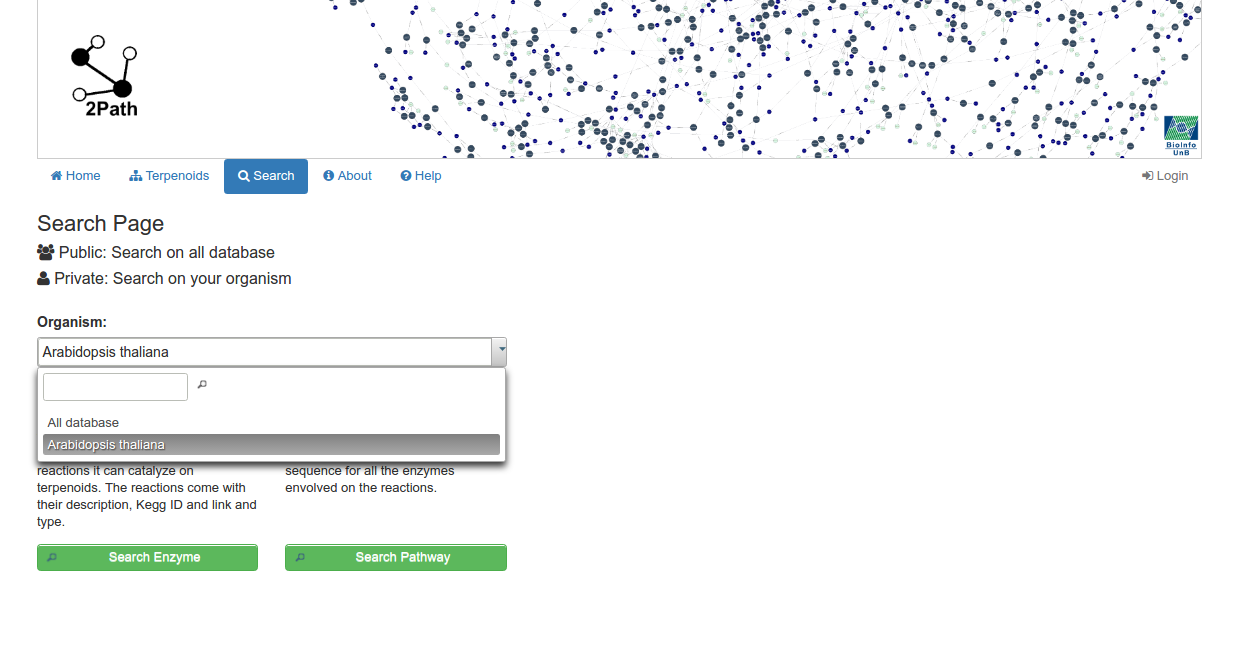
\includegraphics[width=1\textwidth]{new_search_page.png}
    \caption{}
    \label{fig:new_search_page}
\end{figure}

\begin{figure}[!h]
    \centering
    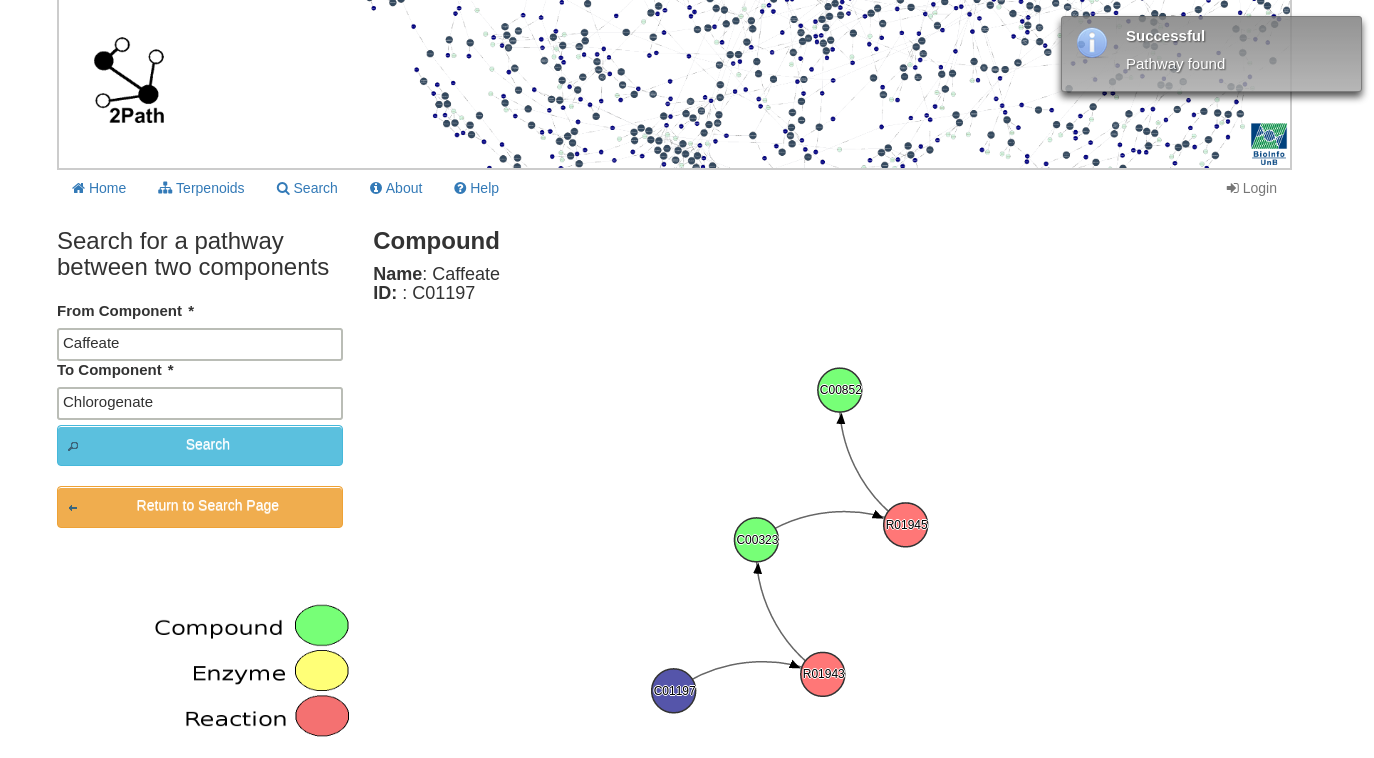
\includegraphics[width=1\textwidth]{new_message_success.png}
    \caption{}
    \label{fig:new_message_success}
\end{figure}

\begin{figure}[!h]
    \centering
    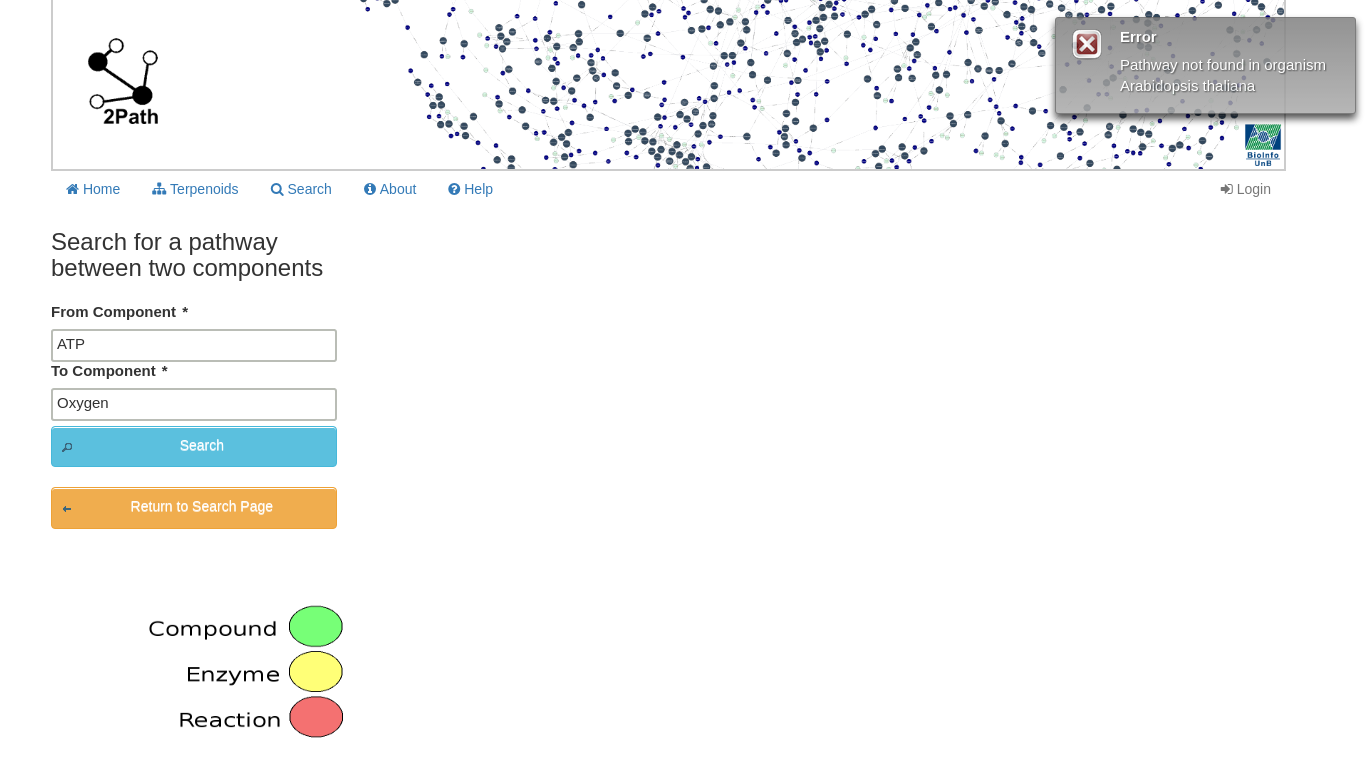
\includegraphics[width=1\textwidth]{new_message_error.png}
    \caption{}
    \label{fig:new_message_error}
\end{figure}

\begin{figure}[!h]
    \centering
    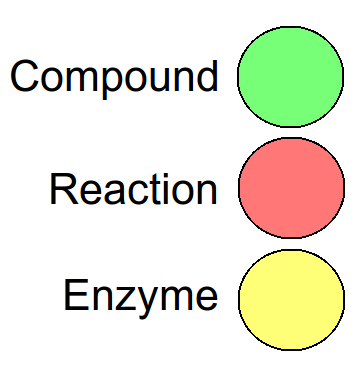
\includegraphics[width=0.2\textwidth]{new_legenda.png}
    \caption{}
    \label{fig:new_legenda}
\end{figure}

\begin{figure}[!h]
    \centering
    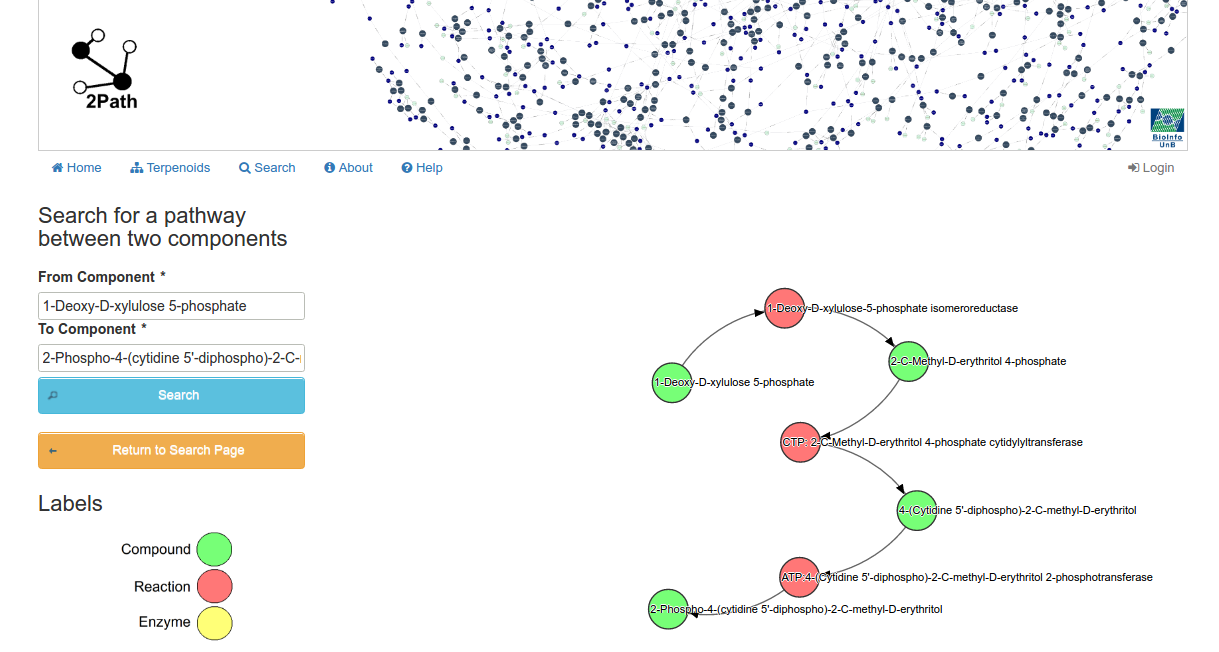
\includegraphics[width=1\textwidth]{new_pathway.png}
    \caption{}
    \label{fig:new_pathway}
\end{figure}

\begin{figure}[!h]
    \centering
    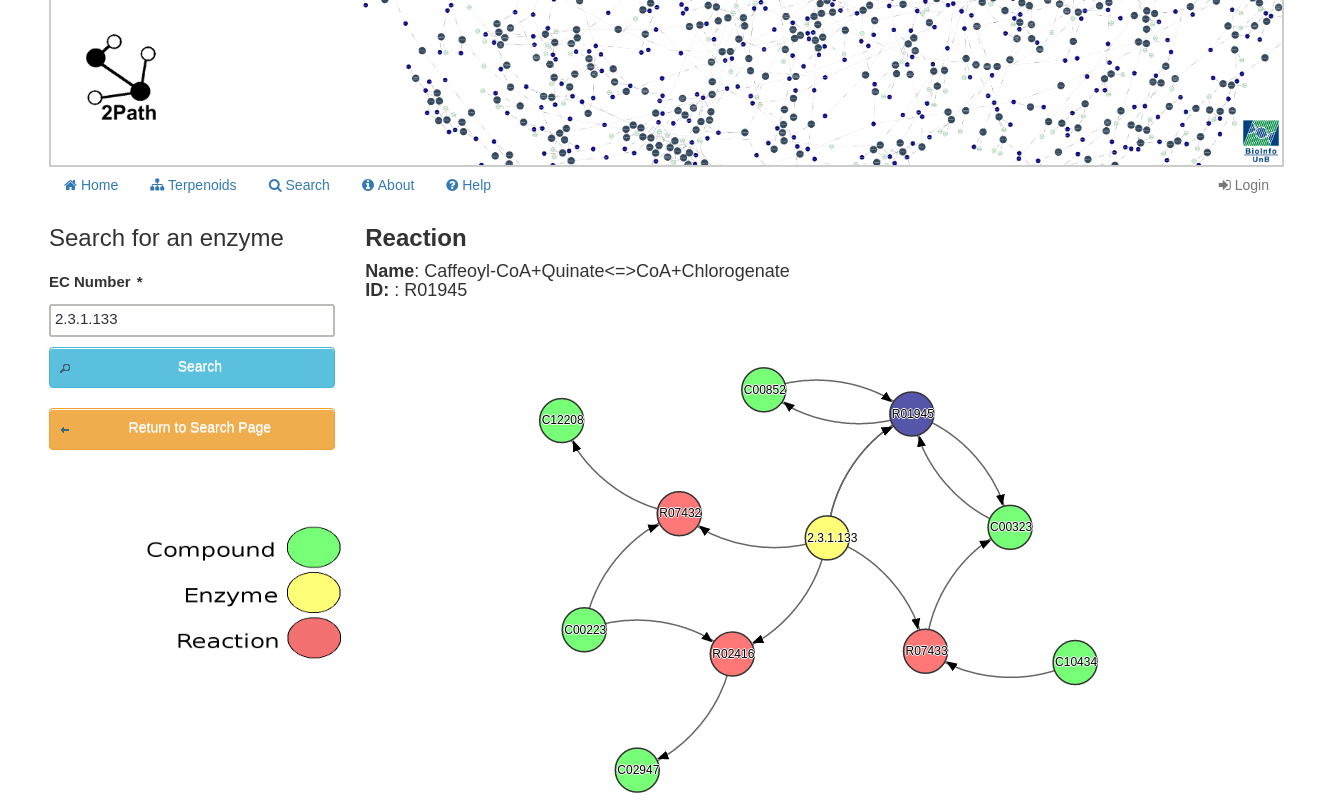
\includegraphics[width=1\textwidth]{new_enzyme_4_catalyses.png}
    \caption{PROBLEMA: ENZIMA PODE CATALIZAR MAIS DE UMA REACAO}
    \label{fig:new_enzyme_4_catalyses}
\end{figure}


